\documentclass{scrartcl}
\usepackage{scrhack}
\usepackage{microtype} % Improves character and word spacing
\setlength{\parindent}{0pt}

\usepackage{graphicx} % Needed to insert images into the document
\graphicspath{{graphics/}} % Sets the default location of pictures
\setkeys{Gin}{width=\linewidth,totalheight=\textheight,keepaspectratio} % Improves figure scaling


\usepackage{fancyvrb} % Allows customization of verbatim environments
\fvset{fontsize=\normalsize} % The font size of all verbatim text can be changed here

\newcommand{\hangp}[1]{\makebox[0pt][r]{(}#1\makebox[0pt][l]{)}} % New command to create parentheses around text in tables which take up no horizontal space - this improves column spacing
\newcommand{\hangstar}{\makebox[0pt][l]{*}} % New command to create asterisks in tables which take up no horizontal space - this improves column spacing

\usepackage{xspace} % Used for printing a trailing space better than using a tilde (~) using the \xspace command

\usepackage{environ}
\makeatletter
\newsavebox{\measure@tikzpicture}
\NewEnviron{scaletikzpicturetowidth}[1]{%
  \def\tikz@width{#1}%
  \def\tikzscale{1}\begin{lrbox}{\measure@tikzpicture}%
  \BODY
  \end{lrbox}%
  \pgfmathparse{#1/\wd\measure@tikzpicture}%
  \edef\tikzscale{\pgfmathresult}%
  \BODY
}
\makeatother

\newcommand{\term}[1]{\textbf{#1}}
\newcommand{\code}[1]{\texttt{#1}}
\newcommand{\plus}{\oplus}
\newcommand{\FI}{\operatorname{FIRST}}
\newcommand{\FO}{\operatorname{FOLLOW}}
\newcommand{\prefix}{\operatorname{prefix}}
\newcommand{\length}{\operatorname{length}}

\newcommand{\dtquote}[1]{"`#1"'}

\newcommand{\al}{\alpha}
\newcommand{\be}{\beta}
\newcommand{\ga}{\gamma}
\newcommand{\de}{\delta}
\newcommand{\ph}{\varphi}
\newcommand{\rh}{\rho}
\newcommand{\ep}{\varepsilon}
\newcommand{\ps}{\psi}
\newcommand{\arrow}{\rightarrow}
\newcommand{\erzeugt}{\ensuremath{\;\underset{rm}{\Longrightarrow}\;}}
\newcommand{\erzeugth}{\ensuremath{\;\underset{rm}{\Longrightarrow}^{*}\;}}



% Commands for grammars
\newcommand{\arbno}[1]{#1\hbox{\rm*}}
\newcommand{\atleastone}[1]{#1\hbox{$^+$}}
\newcommand{\maybe}[1]{#1\hbox{$^?$}}

\newcommand{\tparl}{\tok{(\,}}
\newcommand{\tparr}{\tok{)\,}}
\newcommand{\tcurl}{\tok{\{\,}}
\newcommand{\tcurr}{\tok{\}\,}}
\newcommand{\tbral}{\tok{[\,}}
\newcommand{\tbrar}{\tok{]\,}}
\newcommand{\tsem}{\tok{;\,}}
\newcommand{\tcom}{\tok{,\,}}
\newcommand{\teq}{\tok{=\,}}
\newcommand{\tdot}{\tok{.\,}}

\newcommand{\tint}{\tok{int \,}}
\newcommand{\tpub}{\tok{public \,}}
\newcommand{\tclass}{\tok{class \,}}
\newcommand{\tnew}{\tok{new \,}}
\newcommand{\rid}{\rul{id \,}}
\newcommand{\rstmt}{\rul{Statement}}
\newcommand{\rexp}{\rul{Exp}}
\newcommand{\rtyp}{\rul{Type \,}}
\newcommand{\incurl}[1]{\tcurl #1 \tcurr}
\newcommand{\inparen}[1]{\tparl #1 \tparr}
\newcommand{\inbrac}[1]{\tbral #1 \tbrar}
\newcommand{\inangle}[1]{\ensuremath{\langle #1 \rangle}}

\newcommand{\goesto}{\ensuremath{\to \quad}}



\newcommand{\pl}{\mathcal{P}}
\newcommand{\llvm}{$\nu$LLVM}
\newcommand{\todo}[1]{\textbf{TODO: #1}}
\newcommand{\fixme}[1]{\textbf{FIXME: #1}}

\newcommand{\ls}[1]{\setlength{\baselineskip}{#1\baselineskip}
  \setlength{\itemsep}{0pt}}
\newcommand{\PND}[1]{\operatorname{PND}[#1]}
\newcommand{\DeltaPND}{\Delta\operatorname{PND}}


\usepackage{subfigure}
\usepackage{listings}
\lstset{language=Java}
\lstset{basicstyle=\ttfamily}

\usepackage{amsthm}
\newtheorem{definition}{Definition}
\newtheorem{lemma}{Lemma}
\newtheorem{theorem}{Theorem}


\newenvironment{smallVerbatim}
{\small\verbatim}
{\endverbatim\normalsize}

\newenvironment{smalltt}
{\small\begin{alltt}}
{\end{alltt}\normalsize}

\newcommand{\smallVerbatimInclude}[1]{%
\small\verbatiminput{#1}\normalsize}
\newcommand{\sizeof}[1]{\operatorname{sizeof}(#1)}
\newcommand{\tok}[1]{\textbf{#1}}
\newcommand{\rul}[1]{\textit{#1}}
\newcommand{\successor}[1]{\operatorname{succ}[#1]}
\newcommand{\children}[1]{\operatorname{children}[#1]}
\newcommand{\pred}[1]{\operatorname{pred}[#1]}
\newcommand{\Dom}[1]{\operatorname{dom}[#1]}
\newcommand{\idom}[1]{\operatorname{idom}[#1]}
\newcommand{\dominates}{\succeq}
\newcommand{\dominatesstrict}{\succ}

\usepackage{helvet}
%\usepackage{courier}
\usepackage{verbatim}
\usepackage{booktabs}
%\usepackage[framemethod=TikZ]{mdframed}

\usepackage{amsmath}
\usepackage{amssymb}
%\usepackage{amsthm}
\usepackage{stmaryrd}
\usepackage{ulem}
\usepackage{pgf}

\usepackage{hyperref}
\usepackage{url}



\lstdefinelanguage{javabytecode}
{morekeywords={aaload,aastore,aconst_null,aload,aload_0,aload_1,aload_2,aload_3,anewarray,areturn,arraylength,astore,astore_0,astore_1,astore_2,astore_3,athrow,baload,bastore,bipush,breakpoint,caload,castore,checkcast,d2f,d2i,d2l,dadd,daload,dastore,dcmpg,dcmpl,dconst_0,dconst_1,ddiv,dload,dload_0,dload_1,dload_2,dload_3,dmul,dneg,drem,dreturn,dstore,dstore_0,dstore_1,dstore_2,dstore_3,dsub,dup,dup_x1,dup_x2,dup2,dup2_x1,dup2_x2,f2d,f2i,f2l,fadd,faload,fastore,fcmpg,fcmpl,fconst_0,fconst_1,fconst_2,fdiv,fload,fload_0,fload_1,fload_2,fload_3,fmul,fneg,frem,freturn,fstore,fstore_0,fstore_1,fstore_2,fstore_3,fsub,getfield,getstatic,goto,goto_w,i2b,i2c,i2d,i2f,i2l,i2s,iadd,iaload,iand,iastore,iconst_m1,iconst_0,iconst_1,iconst_2,iconst_3,iconst_4,iconst_5,idiv,if_acmpeq,if_acmpne,if_icmpeq,if_icmpge,if_icmpgt,if_icmple,if_icmplt,if_icmpne,ifeq,ifge,ifgt,ifle,iflt,ifne,ifnonnull,ifnull,iinc,iload,iload_0,iload_1,iload_2,iload_3,impdep1,impdep2,imul,ineg,instanceof,invokedynamic,invokeinterface,invokespecial,invokestatic,invokevirtual,ior,irem,ireturn,ishl,ishr,istore,istore_0,istore_1,istore_2,istore_3,isub,iushr,ixor,jsr,jsr_w,l2d,l2f,l2i,ladd,laload,land,lastore,lcmp,lconst_0,lconst_1,ldc,ldc_w,ldc2_w,ldiv,lload,lload_0,lload_1,lload_2,lload_3,lmul,lneg,lookupswitch,lor,lrem,lreturn,lshl,lshr,lstore,lstore_0,lstore_1,lstore_2,lstore_3,lsub,lushr,lxor,monitorenter,monitorexit,multianewarray,new,newarray,nop,pop,pop2,putfield,putstatic,ret,return,saload,sastore,sipush,swap,tableswitch,wide}
}

\usepackage[T1]{fontenc}
\usepackage[noend]{algorithmic}
\usepackage[latin1]{inputenc}
\usepackage{latexsym}
\usepackage{mathpartir}



\newcommand{\aexp}{\mathit{AExp}}
\newcommand{\powersetof}[1]{\mathbb{P}(#1)}
\newcommand{\variables}{\mathit{Vars}}
\newcommand{\blocks}{\mathit{Blocks}}
\newcommand{\killof}[1]{\mathit{def}(#1)}
\newcommand{\genof}[1]{\mathit{use}(#1)}

\newcommand{\myblue}[1]{\textcolor{blue}{#1}}
\newcommand{\mybluebf}[1]{\myblue{{\bfseries #1}}}

\newcommand{\set}[1]{\{#1\}}
\newcommand{\setcond}[2]{\set{#1\:|\:#2}}

% Commands for typing
\newcommand{\sub}{\prec}
\newcommand{\ct}{\ensuremath{CT}{}}
\newcommand{\tintt}{\mathtt{int}}
\newcommand{\tintarray}{\mathtt{int[]}}
\newcommand{\tboolt}{\mathtt{bool}}
\newcommand{\classDecl}[2]{ \texttt{class } #1 \texttt{ extends } #2 \texttt{ \{ ... \}}}
\newcommand{\ejudge}[2]{\ensuremath{\Gamma \vdash_e #1 : #2}{}}
\newcommand{\ejudgeG}[3]{\ensuremath{#1 \vdash_e #2 : #3}{}}
\newcommand{\sjudge}[1]{\ensuremath{\Gamma \vdash_s #1}{}}
\newcommand{\sjudgeG}[2]{\ensuremath{#1 \vdash_s #2}{}}
\newcommand{\cjudge}[2]{\ensuremath{#1 \vdash_c #2}{}}
\newcommand{\mjudge}[2]{\ensuremath{#1 \vdash_m #2}{}}

\usepackage{textcomp}

%opening
\title{Abstract Syntax Trees}
\author{}

\lstset{basicstyle=\scriptsize\ttfamily,
stringstyle=\ttfamily\color{black!60!red},morekeywords={?,*},
commentstyle=\ttfamily\color{black!60!green},morekeywords={?,*}}

\begin{document}

\maketitle

\tableofcontents

\section{Abstract syntax vs. Concrete syntax}
\label{sec:conc-vs-abs-syntax}

Let $\pl$ be some (programming) language with CFG $\Gamma$ and $p\in \pl$ be a program.
The \term{concrete syntax} of a programming language $\pl$ determines the actual textual representation of programs (incl.\ keywords, separators, etc.).
The syntax tree of $p$ according to $\Gamma$ is the \term{concrete syntax tree of $p$}.

The \term{abstract syntax} of $\pl$ describes the tree structure of
programs in a form that is sufficient and suitable for further processing in subsequent phases.The abstract syntax usually more compact as it focuses on the semantically relevant parts and does not
need to deal with white space, comments, separators, keywords and similar things.
However, to improve error messages for later phases (e.g. during semantical analysis) or debugging, the abstract syntax tree usually also comprises information about source code positions.
A tree for representing a program $p$ according to the abstract syntax is called
the \term{abstract syntax tree of $p$}.

Programming language specifications have to define all aspects of the concrete syntax of the corresponding language, while the abstract syntax is often not specified.

It is possible to use either the concrete or the abstract syntax as interface between the parser and the following phases.

\begin{center}
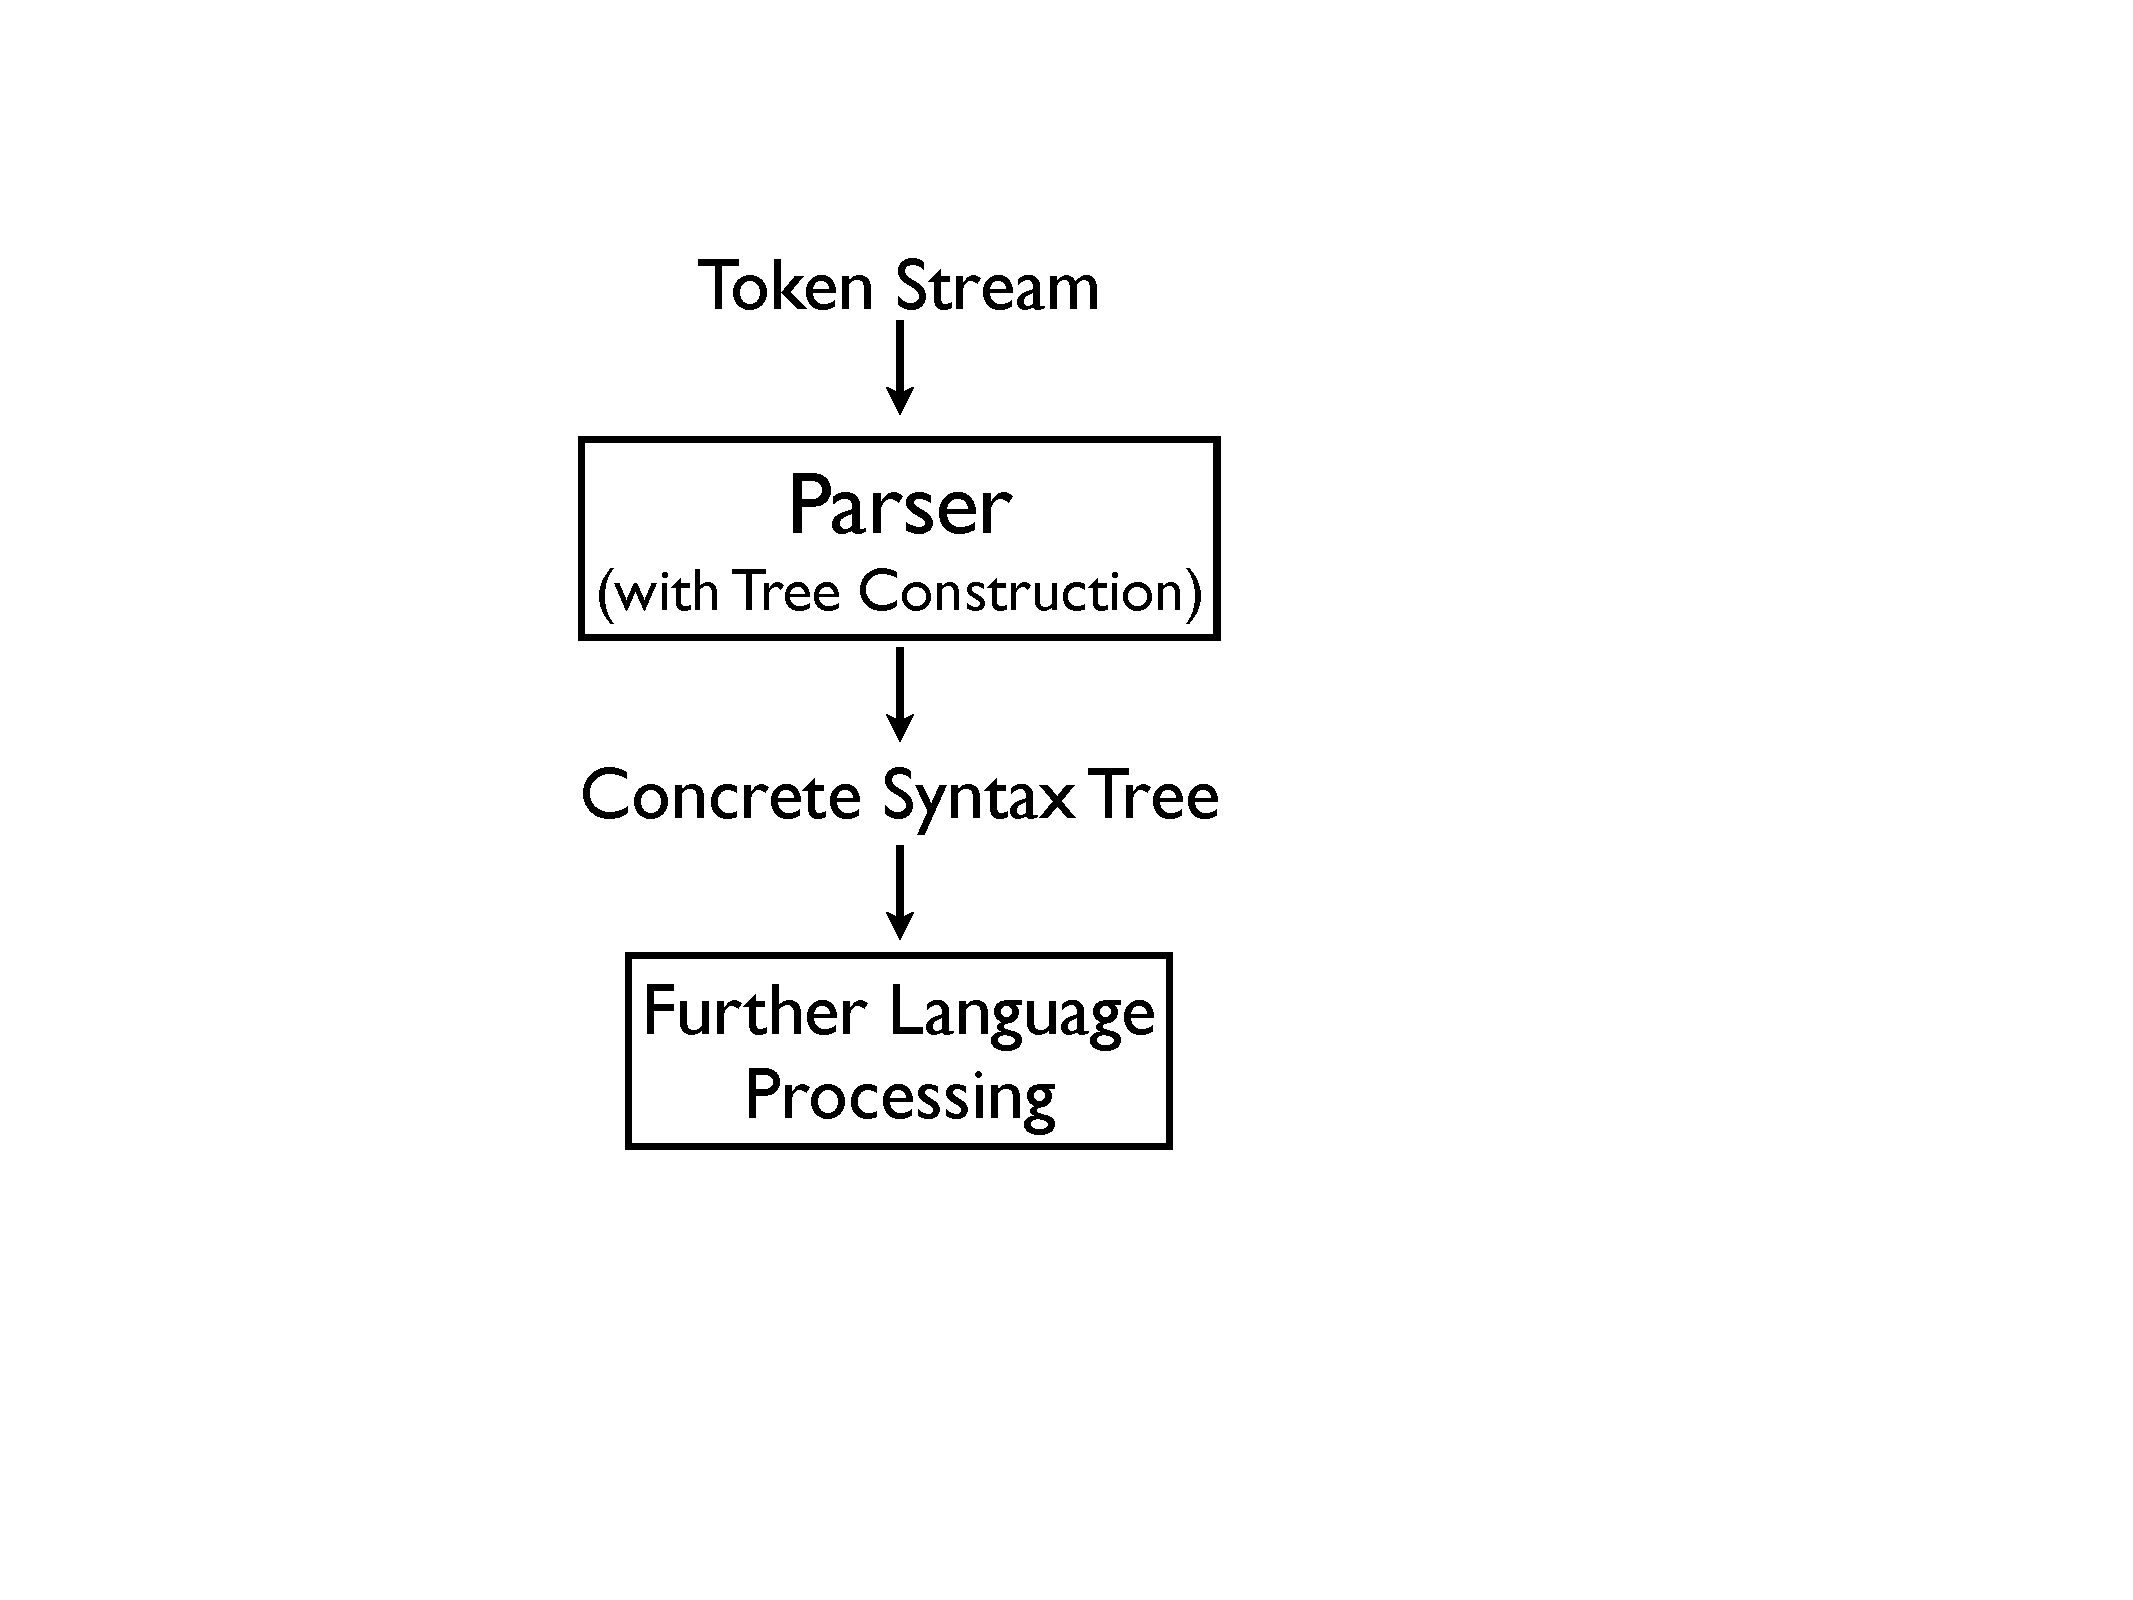
\includegraphics[height=4cm]{conctreeprocess}
\hspace{3cm}
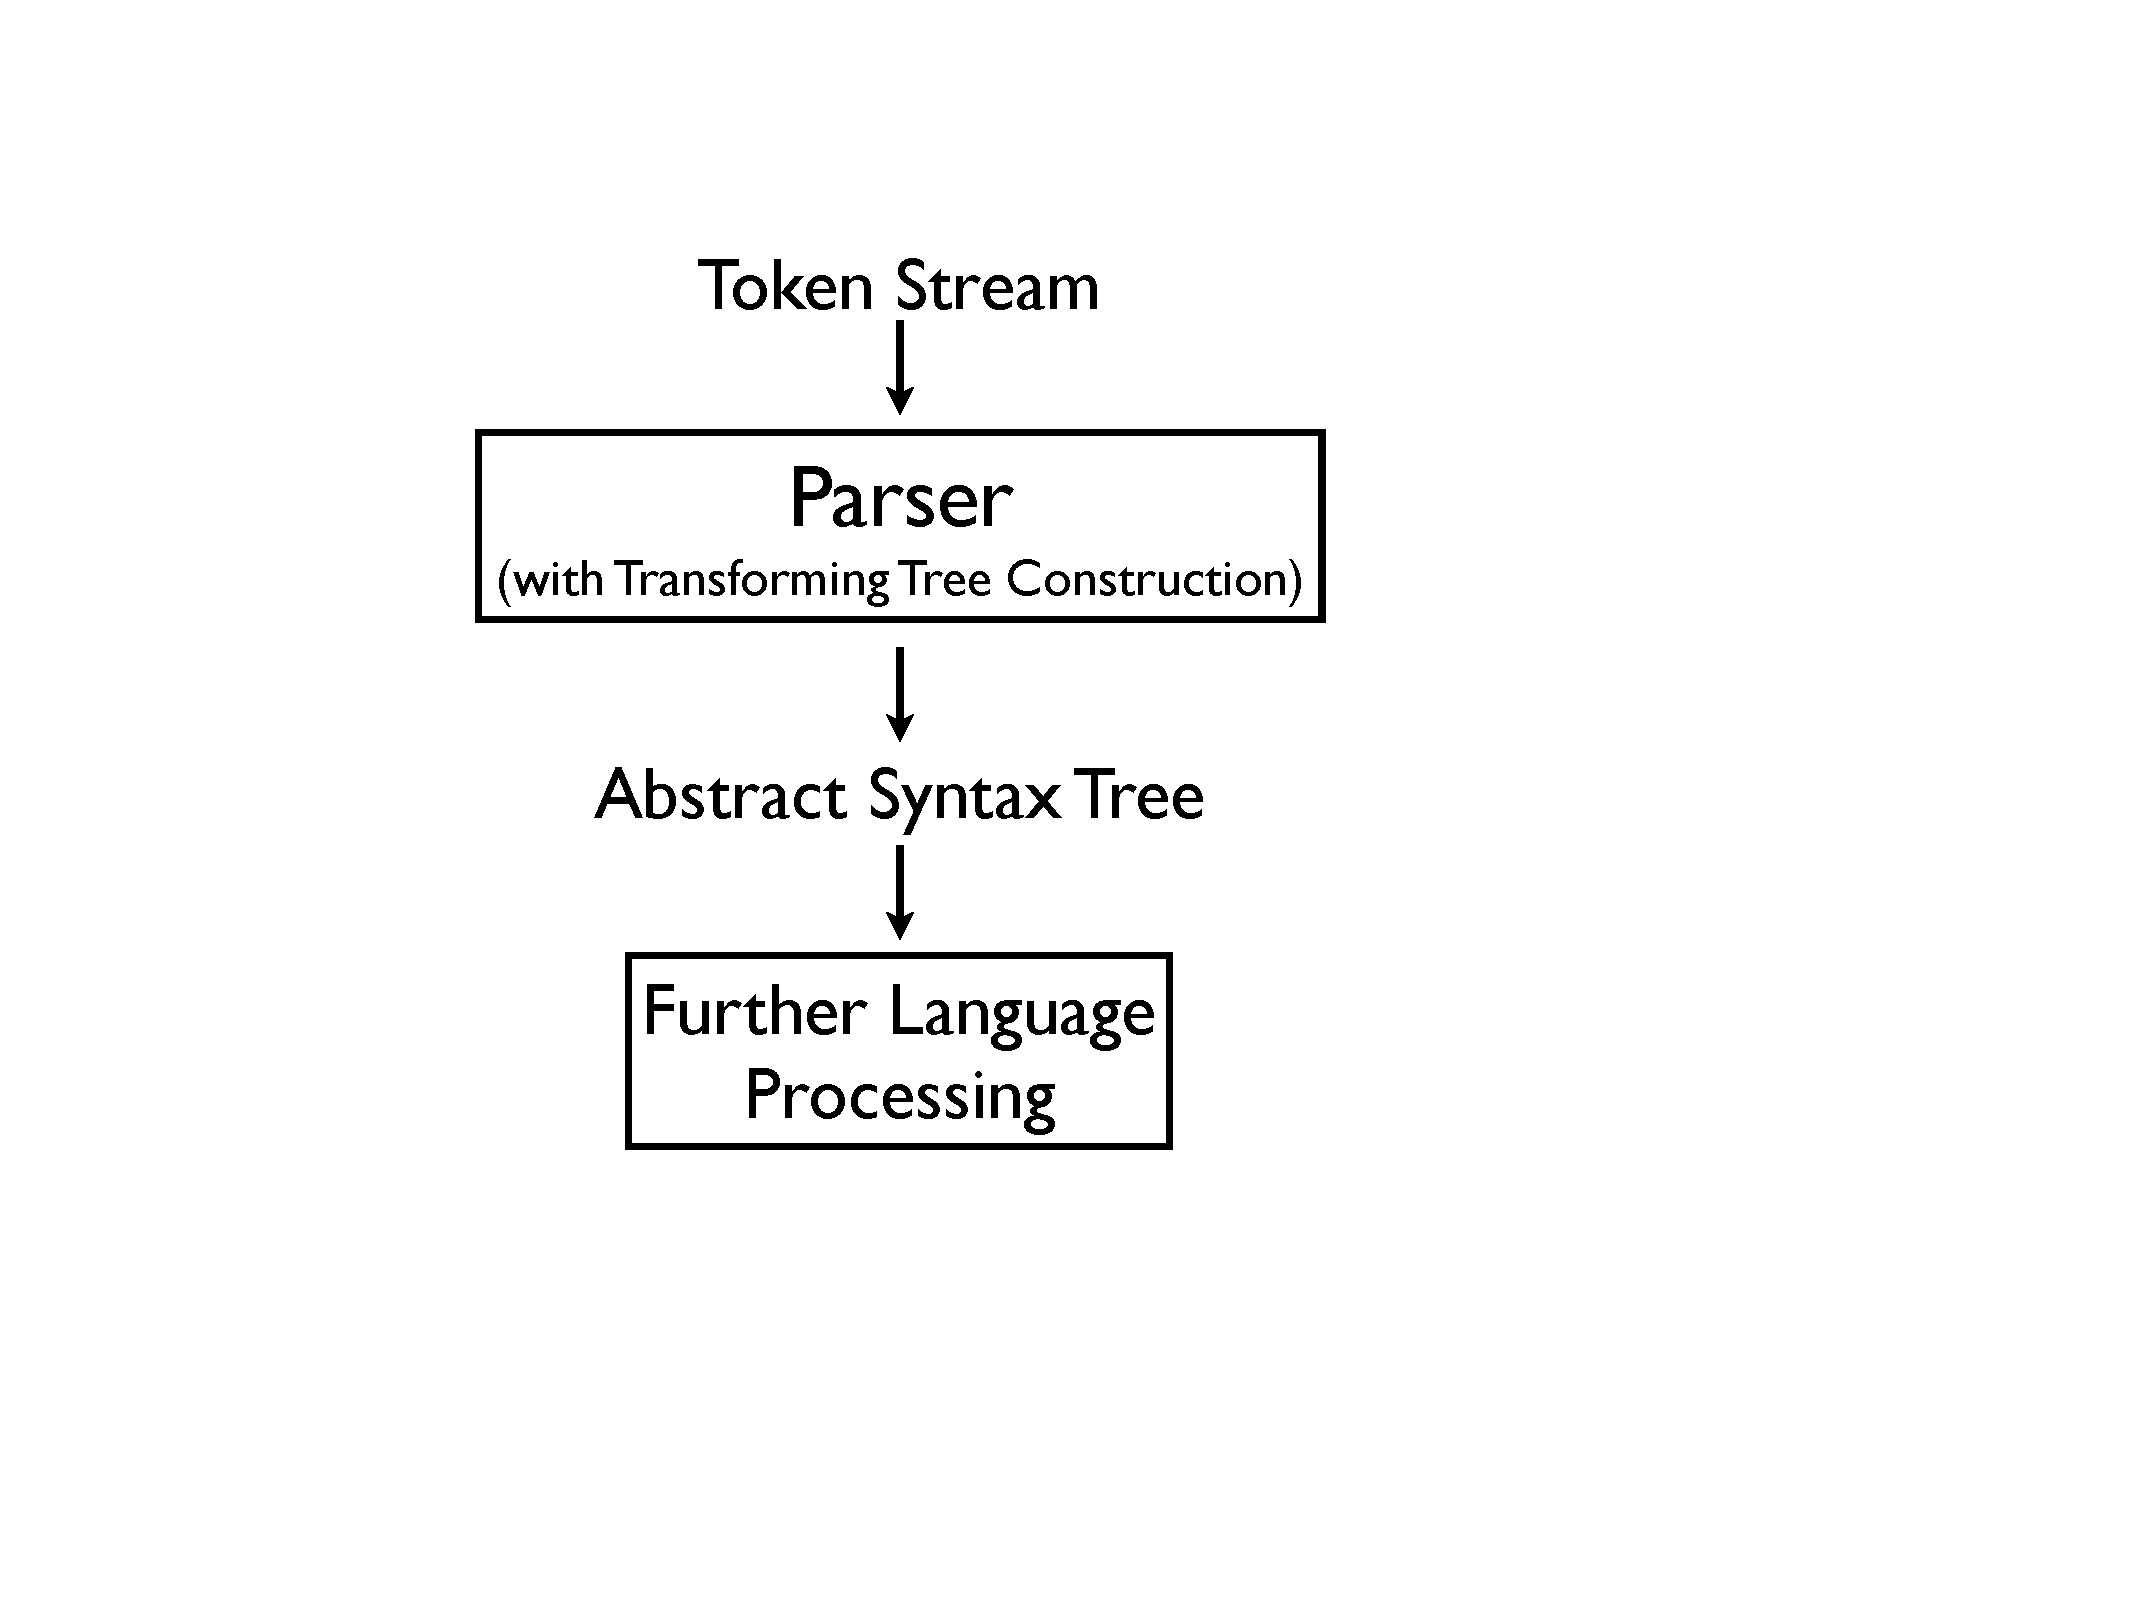
\includegraphics[height=4cm]{abstreeprocess}
\end{center}

When using the concrete syntax, the tree construction can be done
automatically by parser. No additional specification of the abstract syntax is
required, and no translation to an abstract syntax needs to be specified.

However, the simplified structure of the abstract syntax makes it much more feasible for
later phases. Some tools, like SableCC, offer the possibility to specify abstract syntax
and the translation as part of the parser specification.

\paragraph{Example: Concrete vs. abstract syntax}
For the expression language, the concrete syntax can be specified as:
\begin{eqnarray*}
S &\rightarrow& E \# \\
E &\rightarrow& T+E  \;| \; T \\
T &\rightarrow& F * T \; | \; F \\
F &\rightarrow& (E) \; | \; ID
\end{eqnarray*}

A corresponding abstract syntax is usually expressed using algebraic data types (see below):
\begin{lstlisting}[language=Java,basicstyle=\scriptsize\ttfamily]
 Exp = Add | Mult | Ident
 Add  (Exp left, Exp right)
 Mult (Exp left, Exp right)
 Ident(String name)
\end{lstlisting}

For the expression \code{(a + b) * c}, the respective syntax trees are :

%\begin{figure}[h]
\begin{center}
 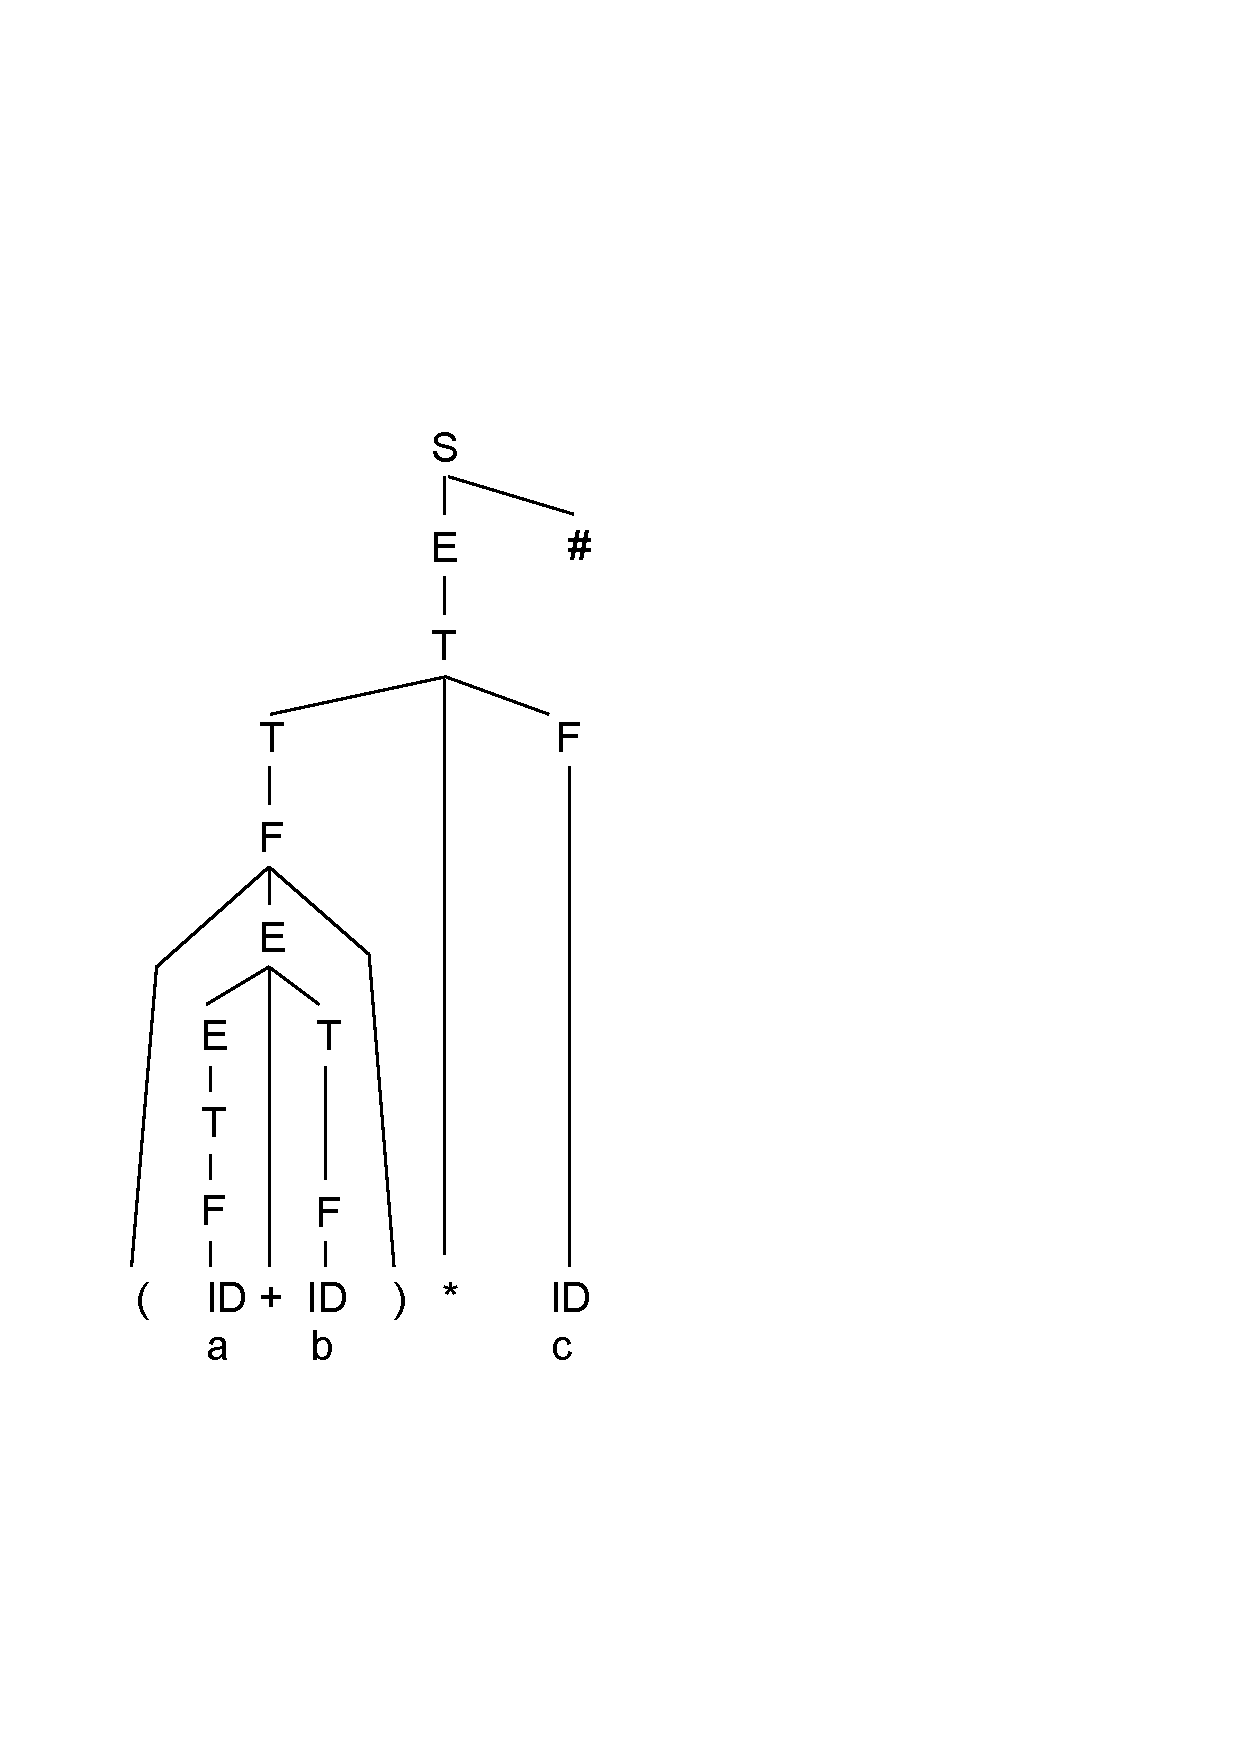
\includegraphics[height=0.4\textwidth]{conctree}
 \hspace{3cm}
 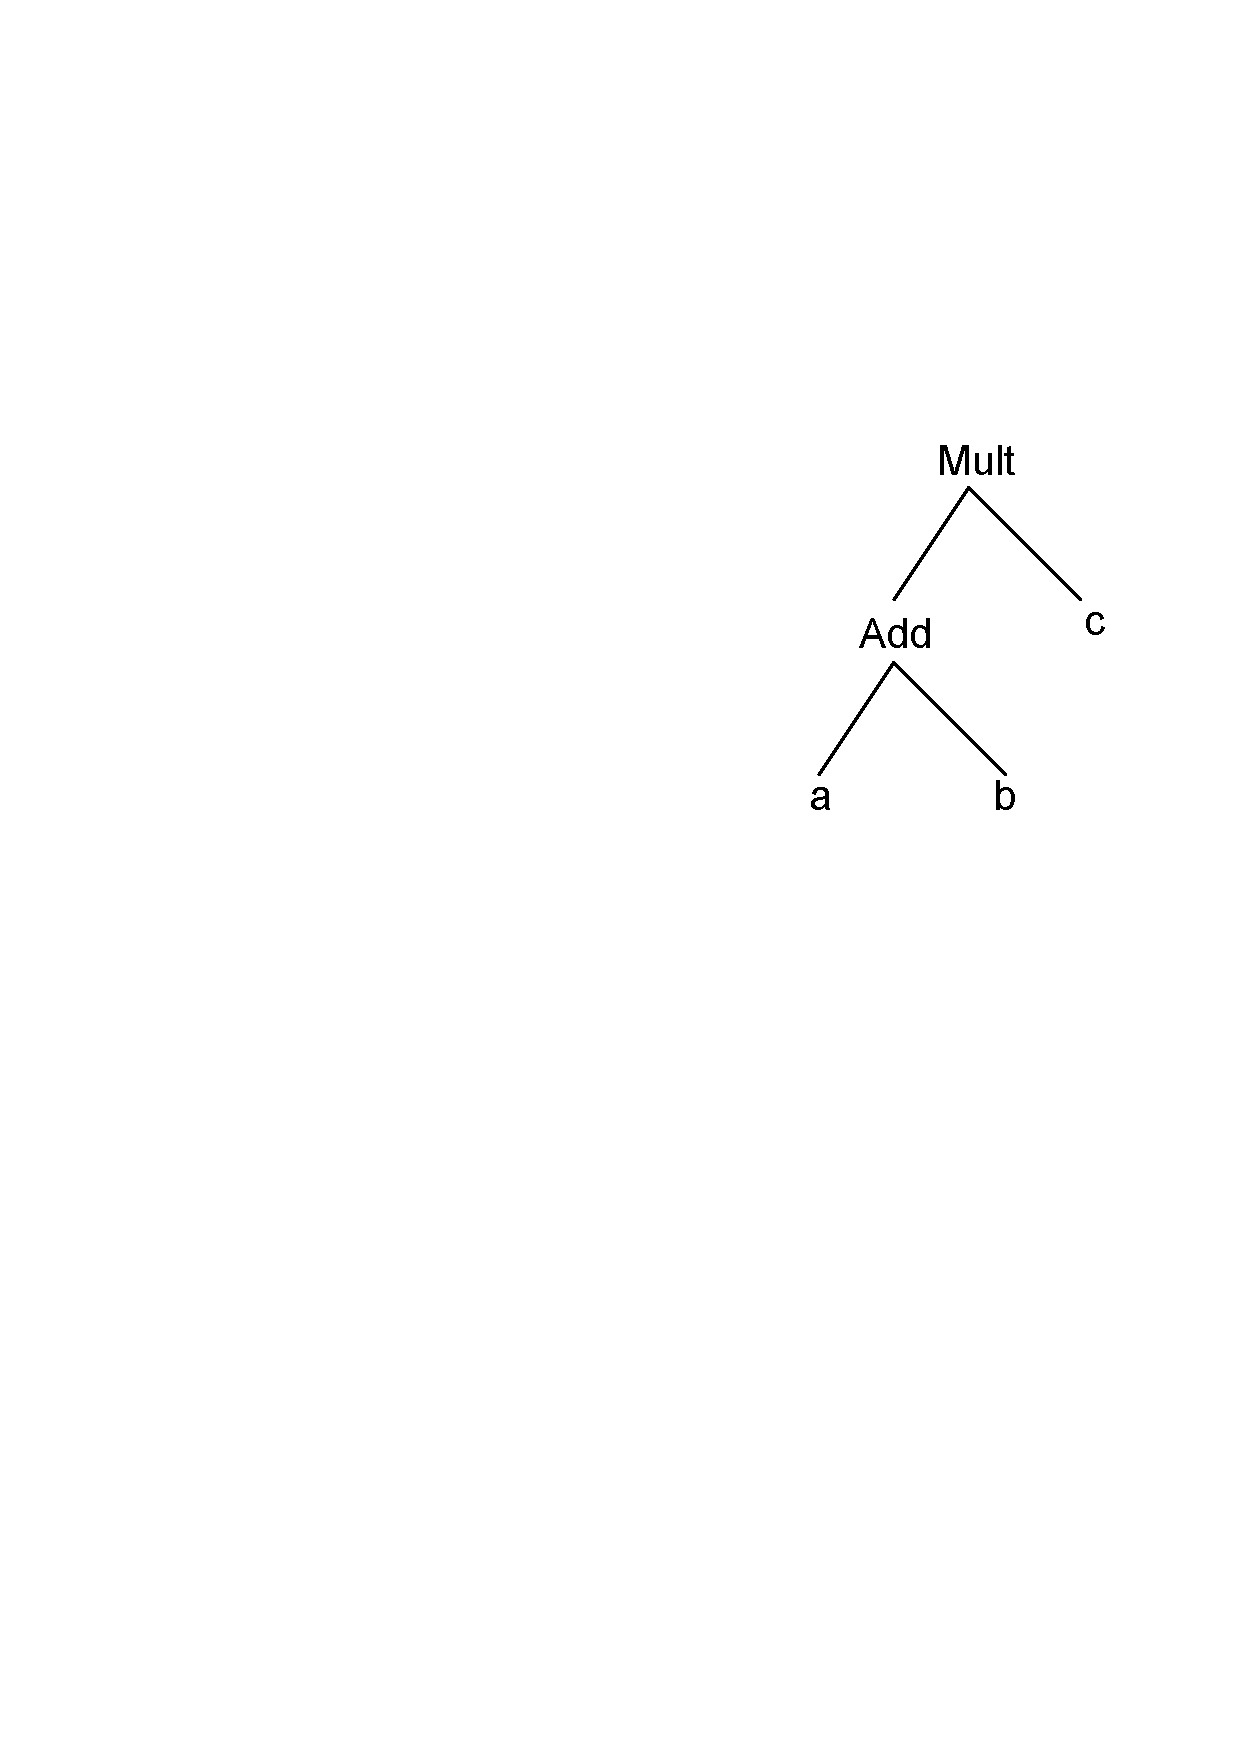
\includegraphics[height=0.2\textwidth]{abstree}
\end{center}
%\caption{Concrete and abstrax syntax tree of expression \code{(a + b) * c}.}
%\label{fig:ex-abs-conc}
%\end{figure}

When transforming from concrete to abstract syntax, the tree structure can usually be simplified. For example, the abstract syntax does not require different nonterminals to reflecting operator precedences. Instead, the precedence is represented in the tree structure itself.

\paragraph{Abstract syntax: Specification and tree construction}
For representing abstract syntax trees, we use algebraic data types.

\begin{definition}
\term{Algebraic data types} are defined using (possibly recursive) sum types and product types.
\begin{itemize}
 \item A sum type $T = T_1 \,|\, T_2 \,|\, \dots \,|\, T_n$ denotes different alternatives for a type $T$.
    Each value of type $T$ falls in exactly one of the cases $T_1$ to $T_n$.

 \item A product type $C(T_1,T_2, \dots, T_m)$ defines a tuple (or record) of values.
    Each value of type $C$ contains values of type $T_1$ to $T_m$ as part of the value.
\end{itemize}
\end{definition}

In most programming languages the notation of sum and product types is combined.
For example the abstract syntax of the expression language (see above) can also be written as follows:

\begin{lstlisting}[language=Java,basicstyle=\scriptsize\ttfamily]
 Exp = Add(Exp left, Exp right)
     | Mult(Exp left, Exp right)
     | Ident(String name)
\end{lstlisting}

Algebraic data types provide a very compact form for type declaration.
They are syntactically supported in many specification languages (e.g. OBJ3, SableCC, Katja, ...).
Further, they are directly supported by a number of functional languages and have a canonical implementation in object-oriented languages:

\begin{itemize}
 \item A sum type $T = T_1 \,|\, T_2 \,|\, \dots \,|\, T_n$ is represented as an abstract class or interface $T$ with concrete subclasses $T_1$ to $T_n$.
 \item A product type $C(T_1,T_2, \dots, T_m)$ is represented by a class with fields of type $T_1$ to $T_m$.
\end{itemize}

The abstract syntax for the expression language (see above) can be represented with the following Java classes:

\begin{lstlisting}[language=Java,basicstyle=\scriptsize\ttfamily]
public abstract class Exp {
    // ...
}
class Add extends Exp {
    private Exp left;
    private Expr right;
    // ...
}
public class Mult extends Exp {
    private Exp left;
    private Expr right;
    // ...
}
public class Ident extends Exp {
    private String name;
    // ...
}
\end{lstlisting}

\section{Abstract Syntax Tree Generation}

In the exercises we generate Java classes and interfaces from a short description of the AST structure.
The description of abstract syntax trees we use consists of three different constructs.

\begin{itemize}
 \item \textbf{Product types} (or ``Constructors'') have a name and a list of parameters. For example an if-statement consists of an expression for the condition, and two statements for the then- and else-branches and would be written as:


\begin{lstlisting}
StmtIf(Expr condition, Statement ifTrue, Statement ifFalse)
\end{lstlisting}

 \item \textbf{Lists} have a name and an element type.
  For example a block-statement is a list of \lstinline!Statement!s and would be written as:
\begin{lstlisting}
Block * Statement
\end{lstlisting}

  \item \textbf{Sum types} (or ``case definitions'') also have a name and a list of different cases.
    The different cases are separated by a vertical bar symbol ``|''.
    For example a Statement can be a \lstinline!Block!, a \lstinline!StmtIf!, or a \lstinline!StmtAssign!, which can be written as:

\begin{lstlisting}
Statement = Block | StmtIf | StmtAssign
\end{lstlisting}
\end{itemize}
As a shorthand notation, it is possible to define constructors inside the definition of a sum type, for example:

\begin{lstlisting}
Statement =
    Block
  | StmtIf(Expr condition, Statement ifTrue, Statement ifFalse)
  | StmtAssign(Expr left, Expr right)
\end{lstlisting}


\subsection{Syntax of AST-description}

The syntax of abstract syntax definitions is given by the EBNF grammar below:

\lstset{upquote=true}
\begin{lstlisting}[stringstyle=\ttfamily\color{blue!50!red},morekeywords={?,*}]
spec ::=
    'package' qID
    ('typeprefix:' ID )?
    'abstract syntax:' element*
    'attributes:'     attributeDef*

element ::=
    contructorDef
  | listDef
  | caseDef

contructorDef ::=
    ID '(' (paramDef (',' paramDef )*)? ')'

paramDef ::=
   'ref'? javaType ID

listDef ::=
    ID '*' 'ref'? ID

caseDef ::=
    name=ID '=' choice ('|' choice)*

choice ::=
    ID
  | contructorDef

attributeDef ::=
    ID '.' ID ( '(' (javaType ID (',' javaType ID)*)? ')' )?
    STRVAL?
    'returns' javaType
    'implemented' 'by' qID
    ('circular' qID)?
  | STRVAL? javaType ID '.' ID

javaType ::=
    ('@Nullable')? qID  ('<' javaType  (',' javaType )*  '>')?;

qID ::=
    ID  ('.' ID)*;
\end{lstlisting}

Whitespace and Java-style comments are ignored.

As an example consider the following AST definition for MiniJava:

\begin{lstlisting}[morekeywords={attributes,syntax,typeprefix}]
package minijava.ast

typeprefix: MJ

abstract syntax:

Program(MainClass mainClass, ClassDeclList classDecls)

MainClass(String name, String argsName, Block mainBody)

ClassDecl(String name, Extended extended, VarDeclList fields, MethodDeclList methods)

Extended =
    ExtendsNothing()
  | ExtendsClass(String name)

VarDecl(Type type, String name)

MethodDecl(Type returnType, String name, VarDeclList formalParameters, Block methodBody)

MemberDecl =
    VarDecl
  | MethodDecl

Type =
    TypeIntArray()
  | TypeInt()
  | TypeBool()
  | TypeClass(String name)

Statement =
    Block
  | StmtIf(Expr condition, Statement ifTrue, Statement ifFalse)
  | StmtWhile(Expr condition, Statement loopBody)
  | StmtReturn(Expr result)
  | StmtPrint(Expr printed)
  | VarDecl
  | StmtExpr(Expr expr)
  | StmtAssign(Expr left, Expr right)

Expr =
    ExprBinary(Expr left, Operator operator, Expr right)
  | ExprUnary(UnaryOperator unaryOperator, Expr expr)
  | ArrayLookup(Expr arrayExpr, Expr arrayIndex)
  | ArrayLength(Expr arrayExpr)
  | FieldAccess(Expr receiver, String fieldName)
  | MethodCall(Expr receiver, String methodName, ExprList arguments)
  | BoolConst(boolean boolValue)
  | VarUse(String varName)
  | Number(int intValue)
  | ExprThis()
  | ExprNull()
  | NewIntArray(Expr arraySize)
  | NewObject(String className)
  | Read()

Operator =
    And()
  | Plus()
  | Minus()
  | Times()
  | Div()
  | Less()
  | Equals()

UnaryOperator =
    UnaryMinus()
  | Negate()


// List types
ClassDeclList * ClassDecl
VarDeclList * VarDecl
MethodDeclList * MethodDecl
Block * Statement
ExprList * Expr

attributes:

"information about the source code"
frontend.SourcePosition Element.sourcePosition
\end{lstlisting}

\subsection{Running the Generator}

The main class of the generator is \lstinline!asg.Main!.
The program accepts two arguments: First the filepath to the AST-specification file and second the filepath to the output folder.

Usually the tool will be run from a build-tool.
For example the following task can be used with Gradle:

\begin{lstlisting}
task genAst {
    description = 'Compile java cup specifications'
    fileTree(dir: 'src/main/java', include:'**/*.ast').each { file ->

        Pattern PACKAGE_PATTERN = Pattern.compile("package\\s+(\\S+)\\s*;");
        String fileContents = file.text

        Matcher matcher = PACKAGE_PATTERN.matcher(fileContents);
        String packageName = "";
        if (matcher.find()) {
            packageName = matcher.group(1);
        }

        String targetDir = "$genDir/" + packageName.replace(".", "/")

        inputs.file(file)
        outputs.dir(targetDir)

        doLast {
            javaexec {
                classpath configurations.compileOnly
                main = "asg.Main"
                args = [file, targetDir]
            }
        }
    }
}
\end{lstlisting}




\subsection{Generated Code}

In the specification it is possible to define a ``typeprefix''.
If a typeprefix is given, it will be added to the name of every generated type.


\subsubsection{The Factory class}
\label{Factory}

A factory class is generated, which contains static methods to create instances of every concrete type.

The name of the factory class is equal to the given typeprefix, or equal to the last part of the package name if no typeprefix is given.

For every constructor definition, a static method is generated, which constructs a new instance of the type.
The signature of the constructor is equivalent to the constructor definition in the specification.

For every list definition, two static methods are created:
One method takes any number of list elements and constructs a list containing these elements.
The other method takes an \lstinline!Iterable! of the elements and uses the elements contained in the \lstinline!Iterable!.


For example consider the following Java method:

\begin{lstlisting}
int foo(int x, int y) {
    int z;
    z = (x + y);
    return z;
}
\end{lstlisting}

An abstract syntax tree representing this program can be constructed with the factory methods mentioned above as follows:

\begin{lstlisting}
MJMethodDecl method = MJ.MethodDecl(MJ.TypeInt(), "foo",
        MJ.VarDeclList(MJ.VarDecl(MJ.TypeInt(), "x"), MJ.VarDecl(MJ.TypeInt(), "y")),
        MJ.Block(
                MJ.VarDecl(MJ.TypeInt(), "z"),
                MJ.StmtAssign(MJ.VarUse("z"), MJ.ExprBinary(MJ.VarUse("x"),
                                                  MJ.Plus(), MJ.VarUse("y"))),
                MJ.StmtReturn(MJ.VarUse("z"))
        ));
\end{lstlisting}


It is also possible to add a static import and thus make the construction shorter and more readable:

\begin{lstlisting}
import static minijava.ast.MJ.*;

...
MJMethodDecl method = MethodDecl(TypeInt(), "foo",
        VarDeclList(VarDecl(TypeInt(), "x"), VarDecl(TypeInt(), "y")),
        Block(
                VarDecl(TypeInt(), "z"),
                StmtAssign(VarUse("z"), ExprBinary(VarUse("x"), Plus(), VarUse("y"))),
                StmtReturn(VarUse("z"))
        ));
\end{lstlisting}

\subsubsection{Sum types}

For every sum type an interface type with name \lstinline!typeprefix + name! is generated.
All cases of the sum type are subtypes of the generated interface.

The sum type contains getters and setters for the fields, which are common to all cases.

A sum type provides a \lstinline!match! method to distinguish the different cases (see Section \ref{Matchers}).

\subsubsection{Constructors}

For each constructor definition an interface and a class are generated.
The name of the interface is \lstinline!typeprefix + name!.

The generated class is package private and never accessed from the outside.
For creating instances of the class, the factory class (see Section \ref{Factory}) is used.
Programs should always refer to the interface type.

The generated interface contains getters and setters for all fields given in the constructor definition.

\subsubsection{Lists}

For each list definition an interface and a class are created.
The generated list implements the \lstinline!java.util.List! interface, so all common list methods can be used.

Additionally, the methods \lstinline!void addFront(T t)! and \lstinline!List<T> removeAll()! are provided.

The method \lstinline!removeAll! removes all elements from the list and returns them as a normal Java list.
This is useful for moving elements from one part of the tree to another (see Section \ref{Invariants}).


\subsubsection{The Element interface}

An interface with name \lstinline!typeprefix + "Element"! is generated, which is a supertype of all other generated types.
In general, the Element interface behaves like a sum type, which is the sum of all other types.

The Element interface provides some general methods to work with ASTs:

\begin{lstlisting}
MJElement getParent();
MJElement copy();
int size();
void clearAttributes();
void clearAttributesLocal();
MJElement get(int i);
MJElement set(int i, MJElement newElement);
void setParent(MJElement parent);
void replaceBy(MJElement other);
boolean structuralEquals(MJElement elem);
<T> T match(Matcher<T> s);
void match(MatcherVoid s);
void accept(Visitor v);
\end{lstlisting}

Each element maintains a link to the parent element, where it is used.
The parent element can be accessed using the \lstinline!getParent! method.
The \lstinline!setParent! method should usually not be called manually, except for circumventing the invariant checks (see Section \ref{Invariants}).

The methods \lstinline!size!, \lstinline!get!, and \lstinline!set! provide generic access to the children of an AST node.
The method \lstinline!size! returns the number of children and the \lstinline!get! and \lstinline!set! methods can be used to access the specific children.

The \lstinline!copy! method creates a deep copy of the AST-node. However, it will not copy external types and fields marked as \lstinline!ref! fields.

The \lstinline!replaceBy! method replaces the current AST node with another node.
This method only changes the reference in the parent element.
Other references will still point to the same object.

The \lstinline!structuralEquals! method checks, if the structure of an element is equal to another element.
Two elements are structurally equal, iff they have the same type, if all children are structurally equal, and if all other fields are equal in the sense of Javas \lstinline!Objects.equals!.

Furthermore, the element interface provides \lstinline!match! methods (see Section \ref{Matchers}), an \lstinline!accept! method for visitors (see Section \ref{Visitors}), and methods to clear calculated Attributes (see section \ref{Attributes}).



\subsection{Invariants}
\label{Invariants}

The generated code tries to maintain some invariants, which are supposed to make programming with the ASTs easier:

\begin{enumerate}
 \item No null references:
  The constructors and setters make sure, that no fields are set to \lstinline!null!.
  Therefore the getters for the fields will never return \lstinline!null!.

 \item Tree structure and parents:
  The constructors and setters try to maintain the invariant, that the parent always points to the right element.
  In particular this means, that each element can have at most one parent and thus be used only once.
  So it is not possible to construct ASTs which are not trees.

  More formally the following invariant should always hold for any element $e$:

  \[ (\textit{e.getParent() != null} \longrightarrow (\exists!i \;:\;  0 \leq i < \textit{e.getParent().size()} \;\wedge\; \textit{e.getParent().get(i)} == e )) \]
  \[ \wedge \; (\forall i  \;:\; 0 \leq i < \textit{e.size()} \longrightarrow   \textit{e.get(i).getParent()} == e) \]

  If an element which already has a parent is added to a different part of a tree an \lstinline!Error! with the message ``Cannot change parent of element ...'' is thrown.

  To circumvent this problem, the easiest method is to use the \lstinline!copy! method to create a copy of a tree.
  For lists it is possible to use the \lstinline!removeAll! method to remove the elements from their current parent, before adding them to another parent.
  It is also possible to manually call \lstinline!setParent(null)! on an element before moving, however this might lead to violations of the invariant.





\end{enumerate}

\subsection{Visitors}
\label{Visitors}

A task that often comes up when working with ASTs involves recursively walking the tree to compute some value for the tree.

For example consider the following definition:

\begin{lstlisting}
Expr =
    ExprBinary(Expr left, Operator operator, Expr right)
  | VarUse(String varName)
  | Number(int intValue)

Operator =
    Plus()
  | Times()
\end{lstlisting}

If we want to write code to evaluate an \lstinline!Expr!, we have to distinguish the different cases.
One way to do this in Java is using \lstinline!instanceof! checks and casts, as in the following code:

\begin{lstlisting}
public int evaluate(MJExpr e, Map<String, Integer> varValues) {
    if (e instanceof MJNumber) {
        MJNumber n = (MJNumber) e;
        return n.getIntValue();
    } else if (e instanceof MJVarUse) {
        MJVarUse v = (MJVarUse) e;
        return varValues.get(v);
    } else if (e instanceof  MJExprBinary){
        MJExprBinary b = (MJExprBinary) e;
        int l = evaluate(b.getLeft(), varValues);
        int r = evaluate(b.getRight(), varValues);
        return evaluateOperator(b.getOperator(), l, r);
    }
    throw new Error("unhandled case: " + e);
}
\end{lstlisting}

A problem with the code above is, that it is easy to miss a case or to get one of the casts wrong.
In particular there is no compiler error, when a case is added to the abstract syntax specification later.

The generated code implements the visitor pattern to support these kind of tasks.
A general introduction to the visitor pattern can be found in:

\begin{itemize}
 \item Oliveira, Bruno CdS, Meng Wang, and Jeremy Gibbons. The visitor pattern as a reusable, generic, type-safe component.
 \item E. Gamma and R. Helm. Design Patterns, Elements of Reusable
Object-Oriented Software.
 \item \url{http://en.wikipedia.org/wiki/Visitor_pattern}
\end{itemize}

To implement a Visitor, create a class which extends \lstinline!typeprefix + "Element.DefaultVisitor"!.
This class comes with \lstinline!visit! methods for all concrete cases of the AST that recursively invoke the accept method on all children.
You can just override the \lstinline!visit! methods, which are relevant for the task at hand.

When overriding a \lstinline!visit! method, you can visit the children by calling the \lstinline!visit! method of the super-class.
For more fine-grained control you can instead invoke the \lstinline!accept! methods of child nodes individually.

For example the evaluation from above could be implemented using a Visitor:

\begin{lstlisting}
class Evaluator extends MJElement.DefaultVisitor {

  private Map<String, Integer> varValues;
  private int value;

  public Evaluator(Map<String, Integer> varValues) {
      this.varValues = varValues;
  }

  @Override
  public void visit(MJVarUse varUse) {
      value = varValues.get(varUse.getVarName());
  }

  @Override
  public void visit(MJExprBinary exprBinary) {
      exprBinary.getLeft().accept(this);
      int left = value;
      exprBinary.getRight().accept(this);
      int right = value;
      value = evaluateOperator(exprBinary.getOperator(), left, right);
  }

  @Override
  public void visit(MJNumber number) {
      value = number.getIntValue();
  }
}


public int evaluate(MJExpr e, Map<String, Integer> varValues) {
  e.accept(new Evaluator(varValues));
  return value;
}
\end{lstlisting}

With this principle it is very easy to implement a method, which calculates the set of used variables in an expression:

\begin{lstlisting}
class VariableFinder extends MJElement.DefaultVisitor {
    Set<String> variables = new TreeSet<>();

    @Override
    public void visit(MJVarUse varUse) {
        variables.add(varUse.getVarName());
    }
}

public Set<String> usedVariables(MJExpr e) {
    VariableFinder variableFinder = new VariableFinder();
    e.accept(variableFinder);
    return variableFinder.variables;
}
\end{lstlisting}

Since no fine-grained control over the order of traversing the children is required, we need only override the \lstinline!visit! method for variable usages.

It is also possible to implement the \lstinline!Visitor! using an anonymous class:

\begin{lstlisting}
public Set<String> usedVariables(MJExpr e) {
    Set<String> variables = new TreeSet<>();
    e.accept(new MJElement.DefaultVisitor() {
        @Override
        public void visit(MJVarUse varUse) {
            variables.add(varUse.getVarName());
        }
    });
    return variables;
}
\end{lstlisting}



\subsection{Matchers}
\label{Matchers}

Matchers are special cases of visitors.
Instead of the complete AST, matchers only distinguish between the different cases of a sum type.

Comming back to our evaluation example:
\begin{lstlisting}
public int evaluateOperator(MJOperator operator, int left, int right) {
  if (operator instanceof MJPlus) {
      return left + right;
  } else if (operator instanceof  MJTimes) {
      return left * right;
  }
}
\end{lstlisting}

As an alternative, it is possible to use the \lstinline!match! methods provided by the generated interfaces.
There are two overloads for the \lstinline!match! method: One returns \lstinline!void! and takes a \lstinline!MatcherVoid! and the other expects a \lstinline!Matcher<T>! and returns \lstinline!T!.

The interfaces \lstinline!MatcherVoid! and \lstinline!Matcher<T>! are generated as inner classes for every sum type and for the general \lstinline!Element! type.

To handle the different cases of a sum type \lstinline!X!, we can simply implement the interface \lstinline!X.Matcher<T>! or \lstinline!X.MatcherVoid! and then pass an instance of the matcher to the \lstinline!match! method.
The interface contains a method for every possible case for the sum type and the \lstinline!match! method will call the correct method based on the actual type of the element.

For example the \lstinline!evaluateOperator! method from above could be implemented using a Matcher:

\begin{lstlisting}
private int evaluateOperator(MJOperator operator, int left, int right) {
    return operator.match(new MJOperator.Matcher<Integer>() {

        @Override
        public Integer case_Plus(MJPlus plus) {
            return left + right;
        }

        @Override
        public Integer case_Times(MJTimes times) {
            return left * right;
        }
    });
}
\end{lstlisting}



\subsection{Additional attributes, methods, and fields}
\label{Attributes}

It is possible to extend the generated classes with additional attributes, methods, and fields, which are declared in the specification after ``attributes:''.

\subsubsection{Fields}

An additional field is declared by the syntax:

\begin{lstlisting}
STRVAL? javaType ID '.' ID
\end{lstlisting}

The definition can start with a String which is used for documentation in the generated code.
Afterwards the field type is declared followed by the name of the type where the field should be added.
The name of the field is then given after a dot.
For example the following definition would add a field of type \lstinline!int! named \lstinline!evaluationResult! to the type \lstinline!Expr!:

\begin{lstlisting}
int Expr.evaluationResult
\end{lstlisting}

For each declared field a getter and a setter method are generated.

\subsubsection{Methods}

An additional method is declared using the following syntax:

\begin{lstlisting}
ID '.' ID '(' (javaType ID (',' javaType ID)*)? ')'
    STRVAL?
    'returns' javaType
    'implemented' 'by' qID
\end{lstlisting}

The first identifier is the type, for which the method should be added.
The second identifier is the name of the method, which is followed by a parameter list as in Java.
After the parameter list there can be a string value for documentation.
Then the return type is given after ``\lstinline!returns!''.

The actual implementation of the method must be in a static method.
The fully qualified name of that method is given at the end after ``\lstinline!implemented by!''.

In the generated code, the method is created and the call is forwarded to the given static method.
Overloading can be used to distinguish different cases of sum types.



\subsubsection{Attributes}

An attribute is defined like a method, but without a parameter list:

\begin{lstlisting}
ID '.' ID
    STRVAL?
    'returns' javaType
    'implemented' 'by' qID
\end{lstlisting}

In contrast to a method, an attribute is only evaluated once on the first call.
All subsequent calls use a cached version of the result.
The methods \lstinline!clearAttributes! and \lstinline!clearAttributesLocal! can be used to clear the cache.

If the value of an attribute is requested while it is being calculated, a \lstinline!CyclicDependencyError! will be thrown.



\subsection{Ref fields}
\label{Refs}

For intermediate languages it sometimes make sense to have cross references to other elements in the tree.
For example a variable use in an intermediate language could directly defer to the declaration of the variable instead of just storing the name of the variable, so that it is not necessary to do a second name analysis.

As those references don't obey to the tree structure (there can be many uses of the same variable), they have to be distinguished from other fields.
This can be done by writing \lstinline!ref! in front of the type of a field in a constructor or list definition.
For example:

\begin{lstlisting}
ExprVarAccess(ref Local var)
TypeRefList * ref Type
\end{lstlisting}

For fields marked with \lstinline!ref! the parent invariant is not enforced and the parent is not changed for referenced elements.



\section{Use with Java Cup}

The recommended way to use the generated AST classes with a parser generator like Java CUP is to add a static import like:

\begin{lstlisting}
import minijava.ast.*;
import static minijava.ast.MJ.*;
\end{lstlisting}

With the static import in place, the AST can be constructed in the parser actions, by simply calling the factory methods (See \ref{Factory}).

For example an AST for expressions can be build as follows:

\begin{lstlisting}
expr ::=
        expr:l AND expr:r
            {: RESULT = ExprBinary(l, And(), r); :}
      | expr:l PLUS expr:r
            {: RESULT = ExprBinary(l, Plus(), r); :}
      ...
\end{lstlisting}

When building lists, the usual methods from \lstinline!java.util.List! can be used, as shown in the following example to build  a list of class declarations:

\begin{lstlisting}
classDeclList ::=
        classDecl:c classDeclList:l
            {: RESULT = l; l.add(0, c); :}
      | /* empty */
            {: RESULT = ClassDeclList(); :}
      ;
\end{lstlisting}

Remember, that any valid Java code can be written in the parser actions.
In particular, you can also call your own helper-methods, if more complicated transformations are required.



\end{document}
